\section{Results}
\label{sec:results}

\subsection{The odd pentamer retains a low-energy spin doublet}

At all 100 sampled points with $0<\alpha\leq1$, the isolated-pentamer ground state is an even-reflection-parity spin-$1/2$ doublet.
The lowest excited doublet is odd under reflection, whereas the lowest spin-$3/2$ multiplet is even.
The five-spin unit therefore retains an active half-integer degree of freedom instead of forming a fully quenched singlet cluster.

At $\alpha=0.14$, 0.23, and 0.33, the projected coupling satisfies $\Jeff/\beta=0.4396$, 0.4318, and 0.4189, respectively.
Positive $\beta$ therefore generates an antiferromagnetic effective spin-$1/2$ chain.
The residual between projected and exact ground-state energies scales with powers 1.9689--1.9915 for two coupled pentamers and 1.9483--1.9495 for complete chains with $N=8,12,16$.
The leading correction is consistent with the $O(\beta^2)$ term in Eq.~\eqref{eq:effective}.

\begin{figure*}[t]
  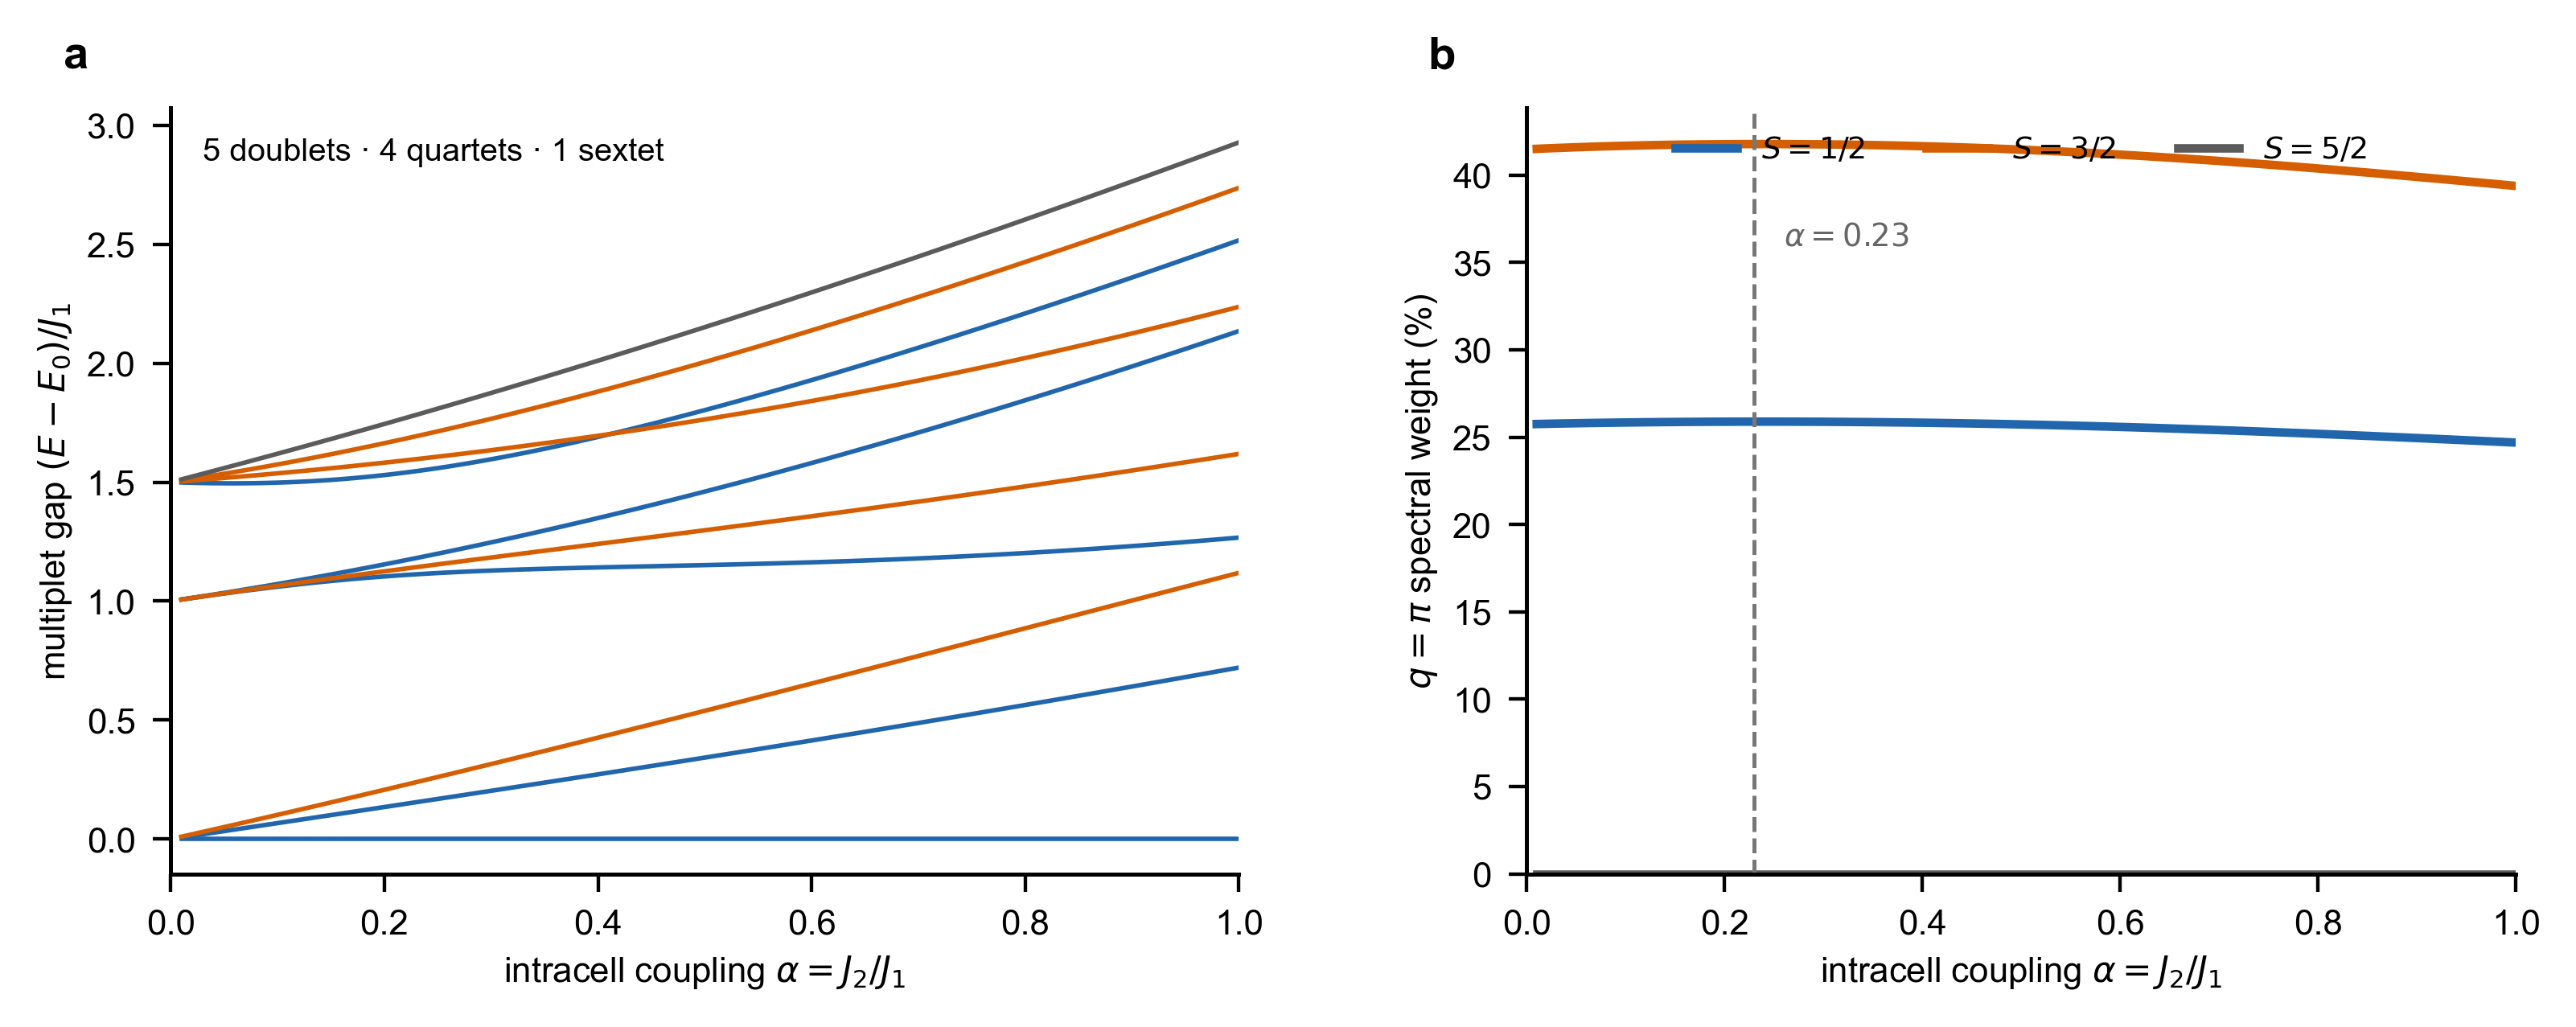
\includegraphics[width=\textwidth]{fig2_multiplet_parity.png}
  \caption{Multiplet flow and the $q=\pi$ parity filter for positive $\alpha$.
  The lowest excited doublet is dark, whereas even-parity spin-$3/2$ multiplets dominate the local inelastic response.}
  \label{fig:multiplets}
\end{figure*}

\subsection{Positive couplings support one resolved effective-chain regime}

The strict positive-region mesh contains 105 accepted records.
Its $L=40,60,80$ finite-size diagnostic does not produce a stable interior crossing.
All accepted interior size differences retain the same sign under leave-one-out and weakest-point audits.
This bounded negative result establishes that the present data resolve no internal boundary in $0\leq\alpha,\beta\leq1$, but it does not prove that every thermodynamic point belongs to one phase.

At $\alpha=0.23$ and weak inter-cell coupling, matched-size entanglement estimators give $\ceff=1.0240$--1.0331 relative to an open spin-$1/2$ Heisenberg-chain oracle.
The comparison uses open chains of $N=8$--$24$ pentamers ($L=40$--$120$) with the same boundary condition and fitting window for both models, and the bond entropy is stable against a doubling of the retained bond dimension (largest relative change $2.4\times10^{-4}$).
Finite-size spin gaps extrapolate close to zero, the correlation envelope has exponents 0.95--0.98, and the static structure factor is dominated by $q=\pi$.
Together, these observables are consistent with a gapless antiferromagnetic effective chain at the tested points~\cite{descloizeaux1962_verified}.
The unmatched absolute $\log L$ fits do not pass an independent quality gate, so the calibrated matched-size ratio is the operative statement; we do not report an unbiased thermodynamic central charge.

\begin{figure*}[t]
  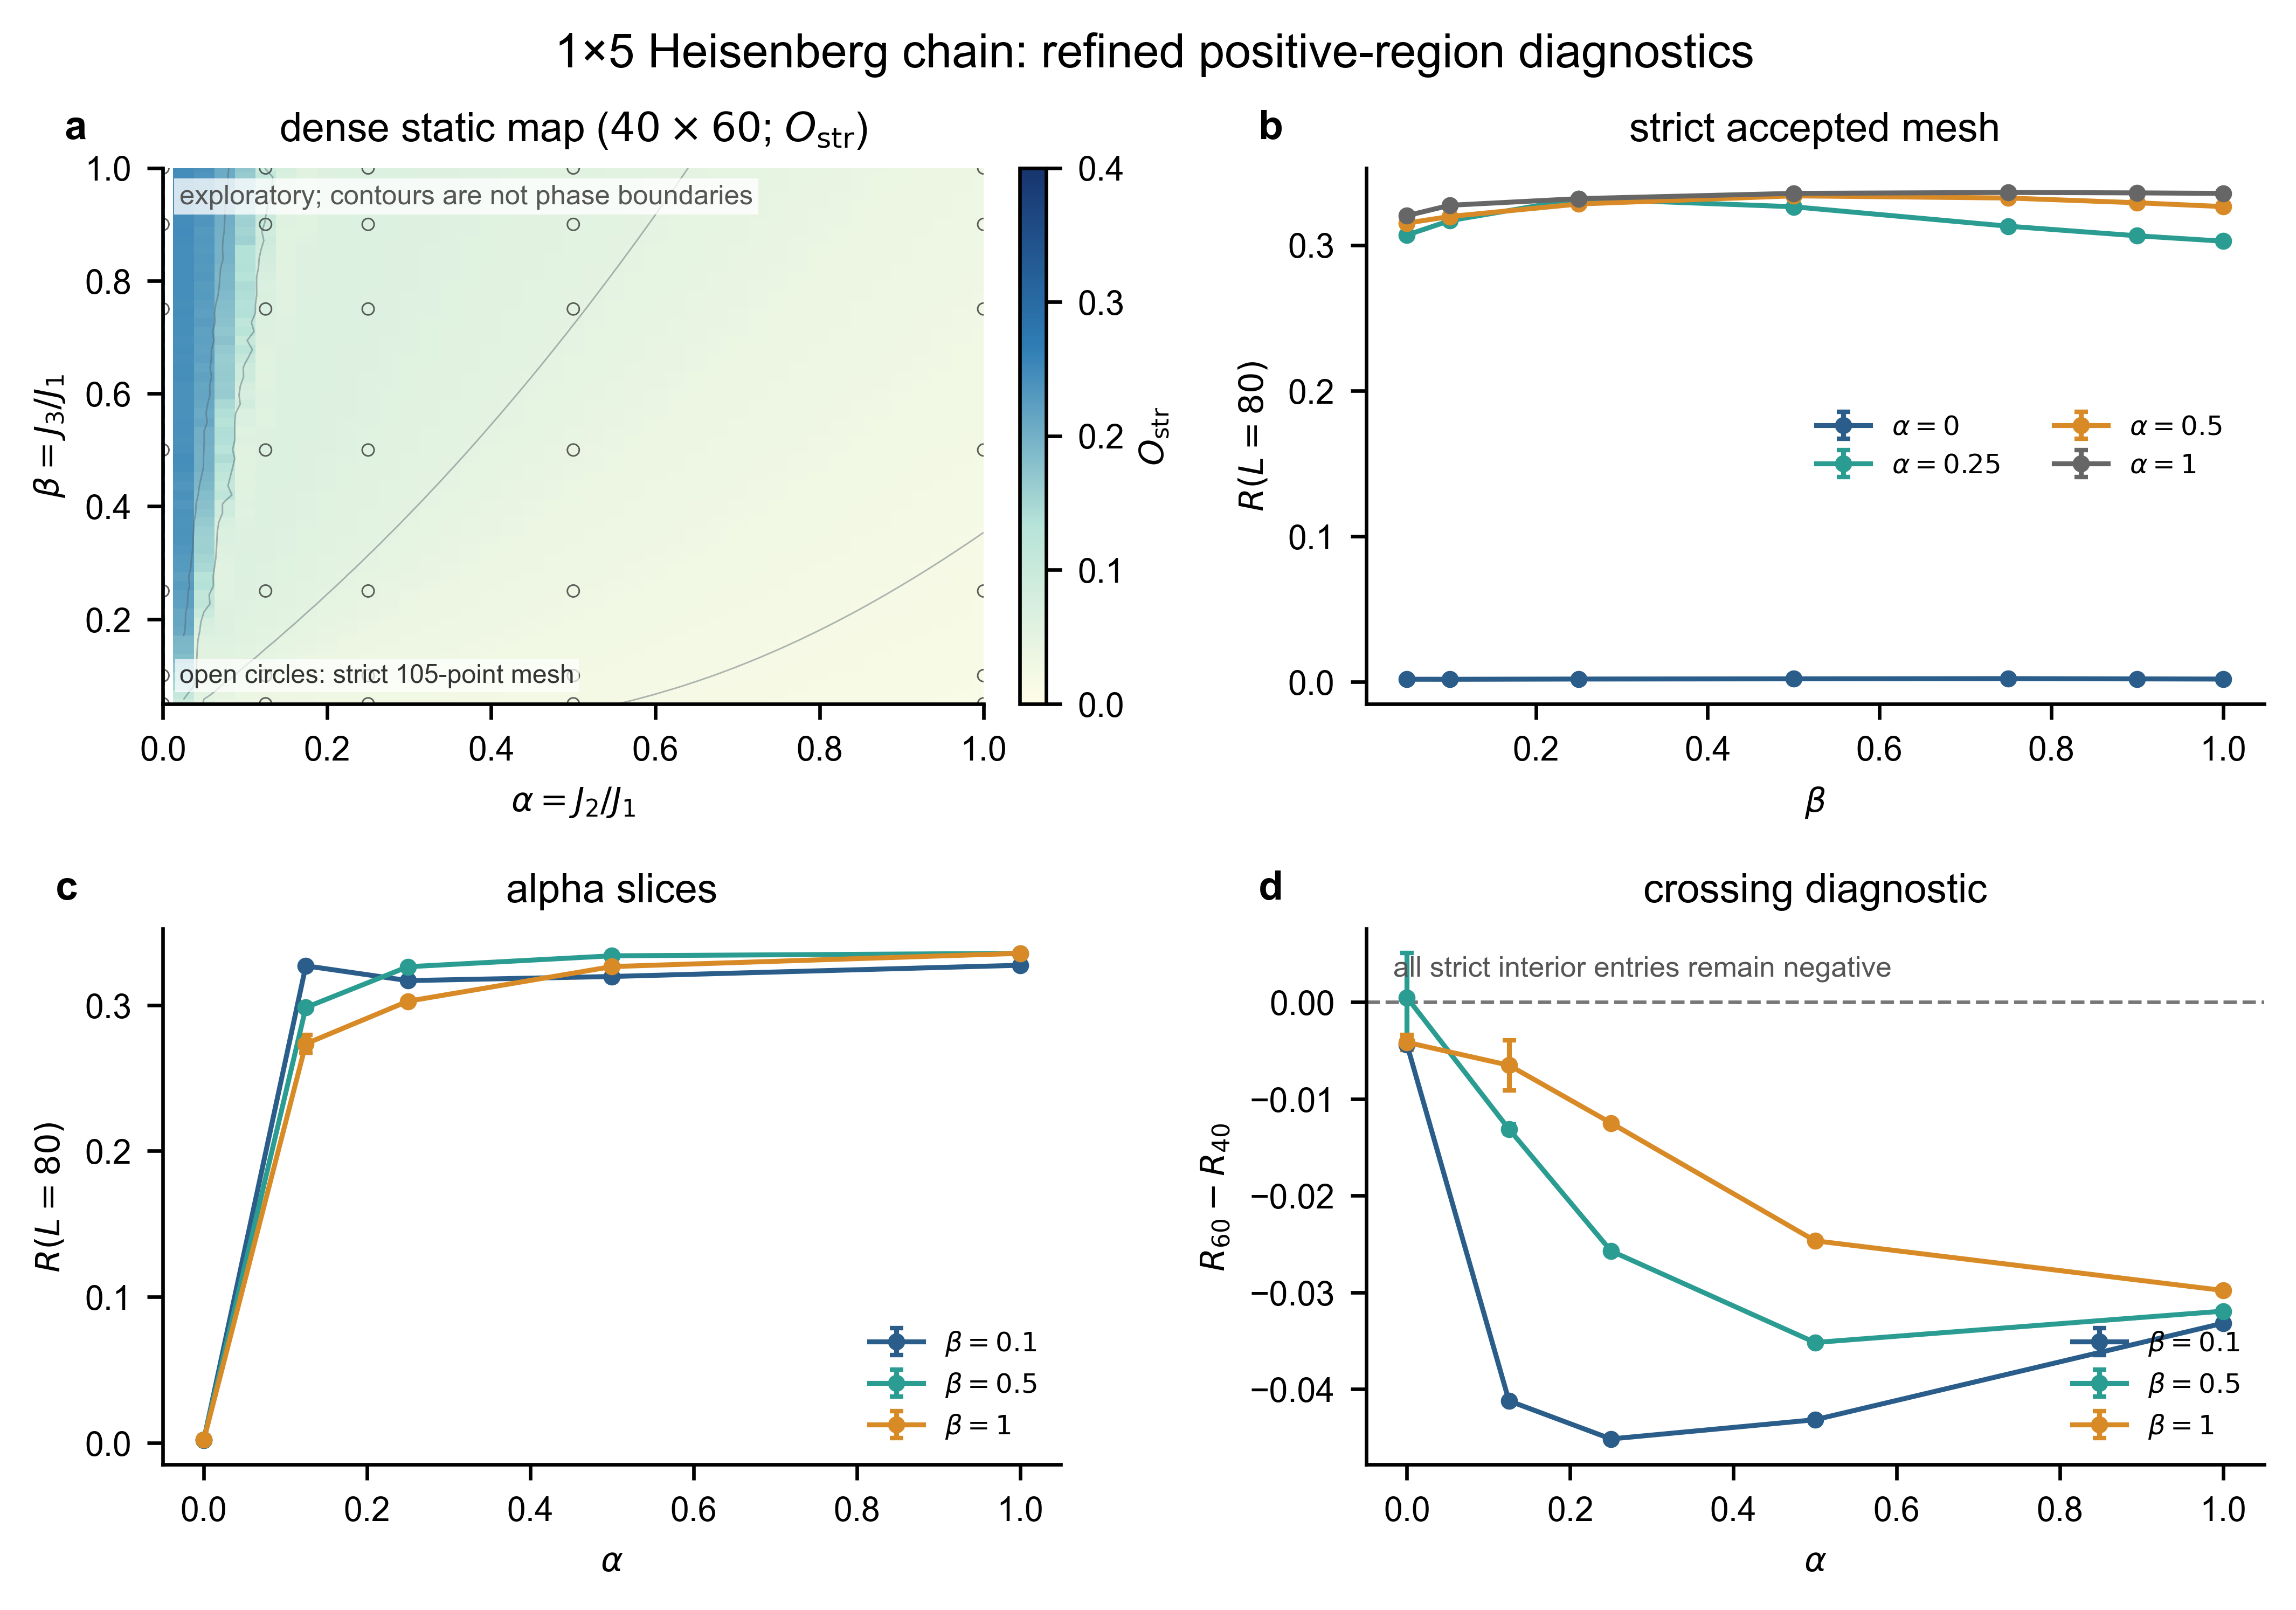
\includegraphics[width=0.98\textwidth]{fig3_positive_static.png}
  \caption{Positive-region ground-state diagnostics.
  The dense map is exploratory, whereas the strict 105-record $L=40,60,80$ mesh supplies the accepted crossing test.
  No stable internal bracket is resolved.}
  \label{fig:positive-static}
\end{figure*}

\begin{figure*}[t]
  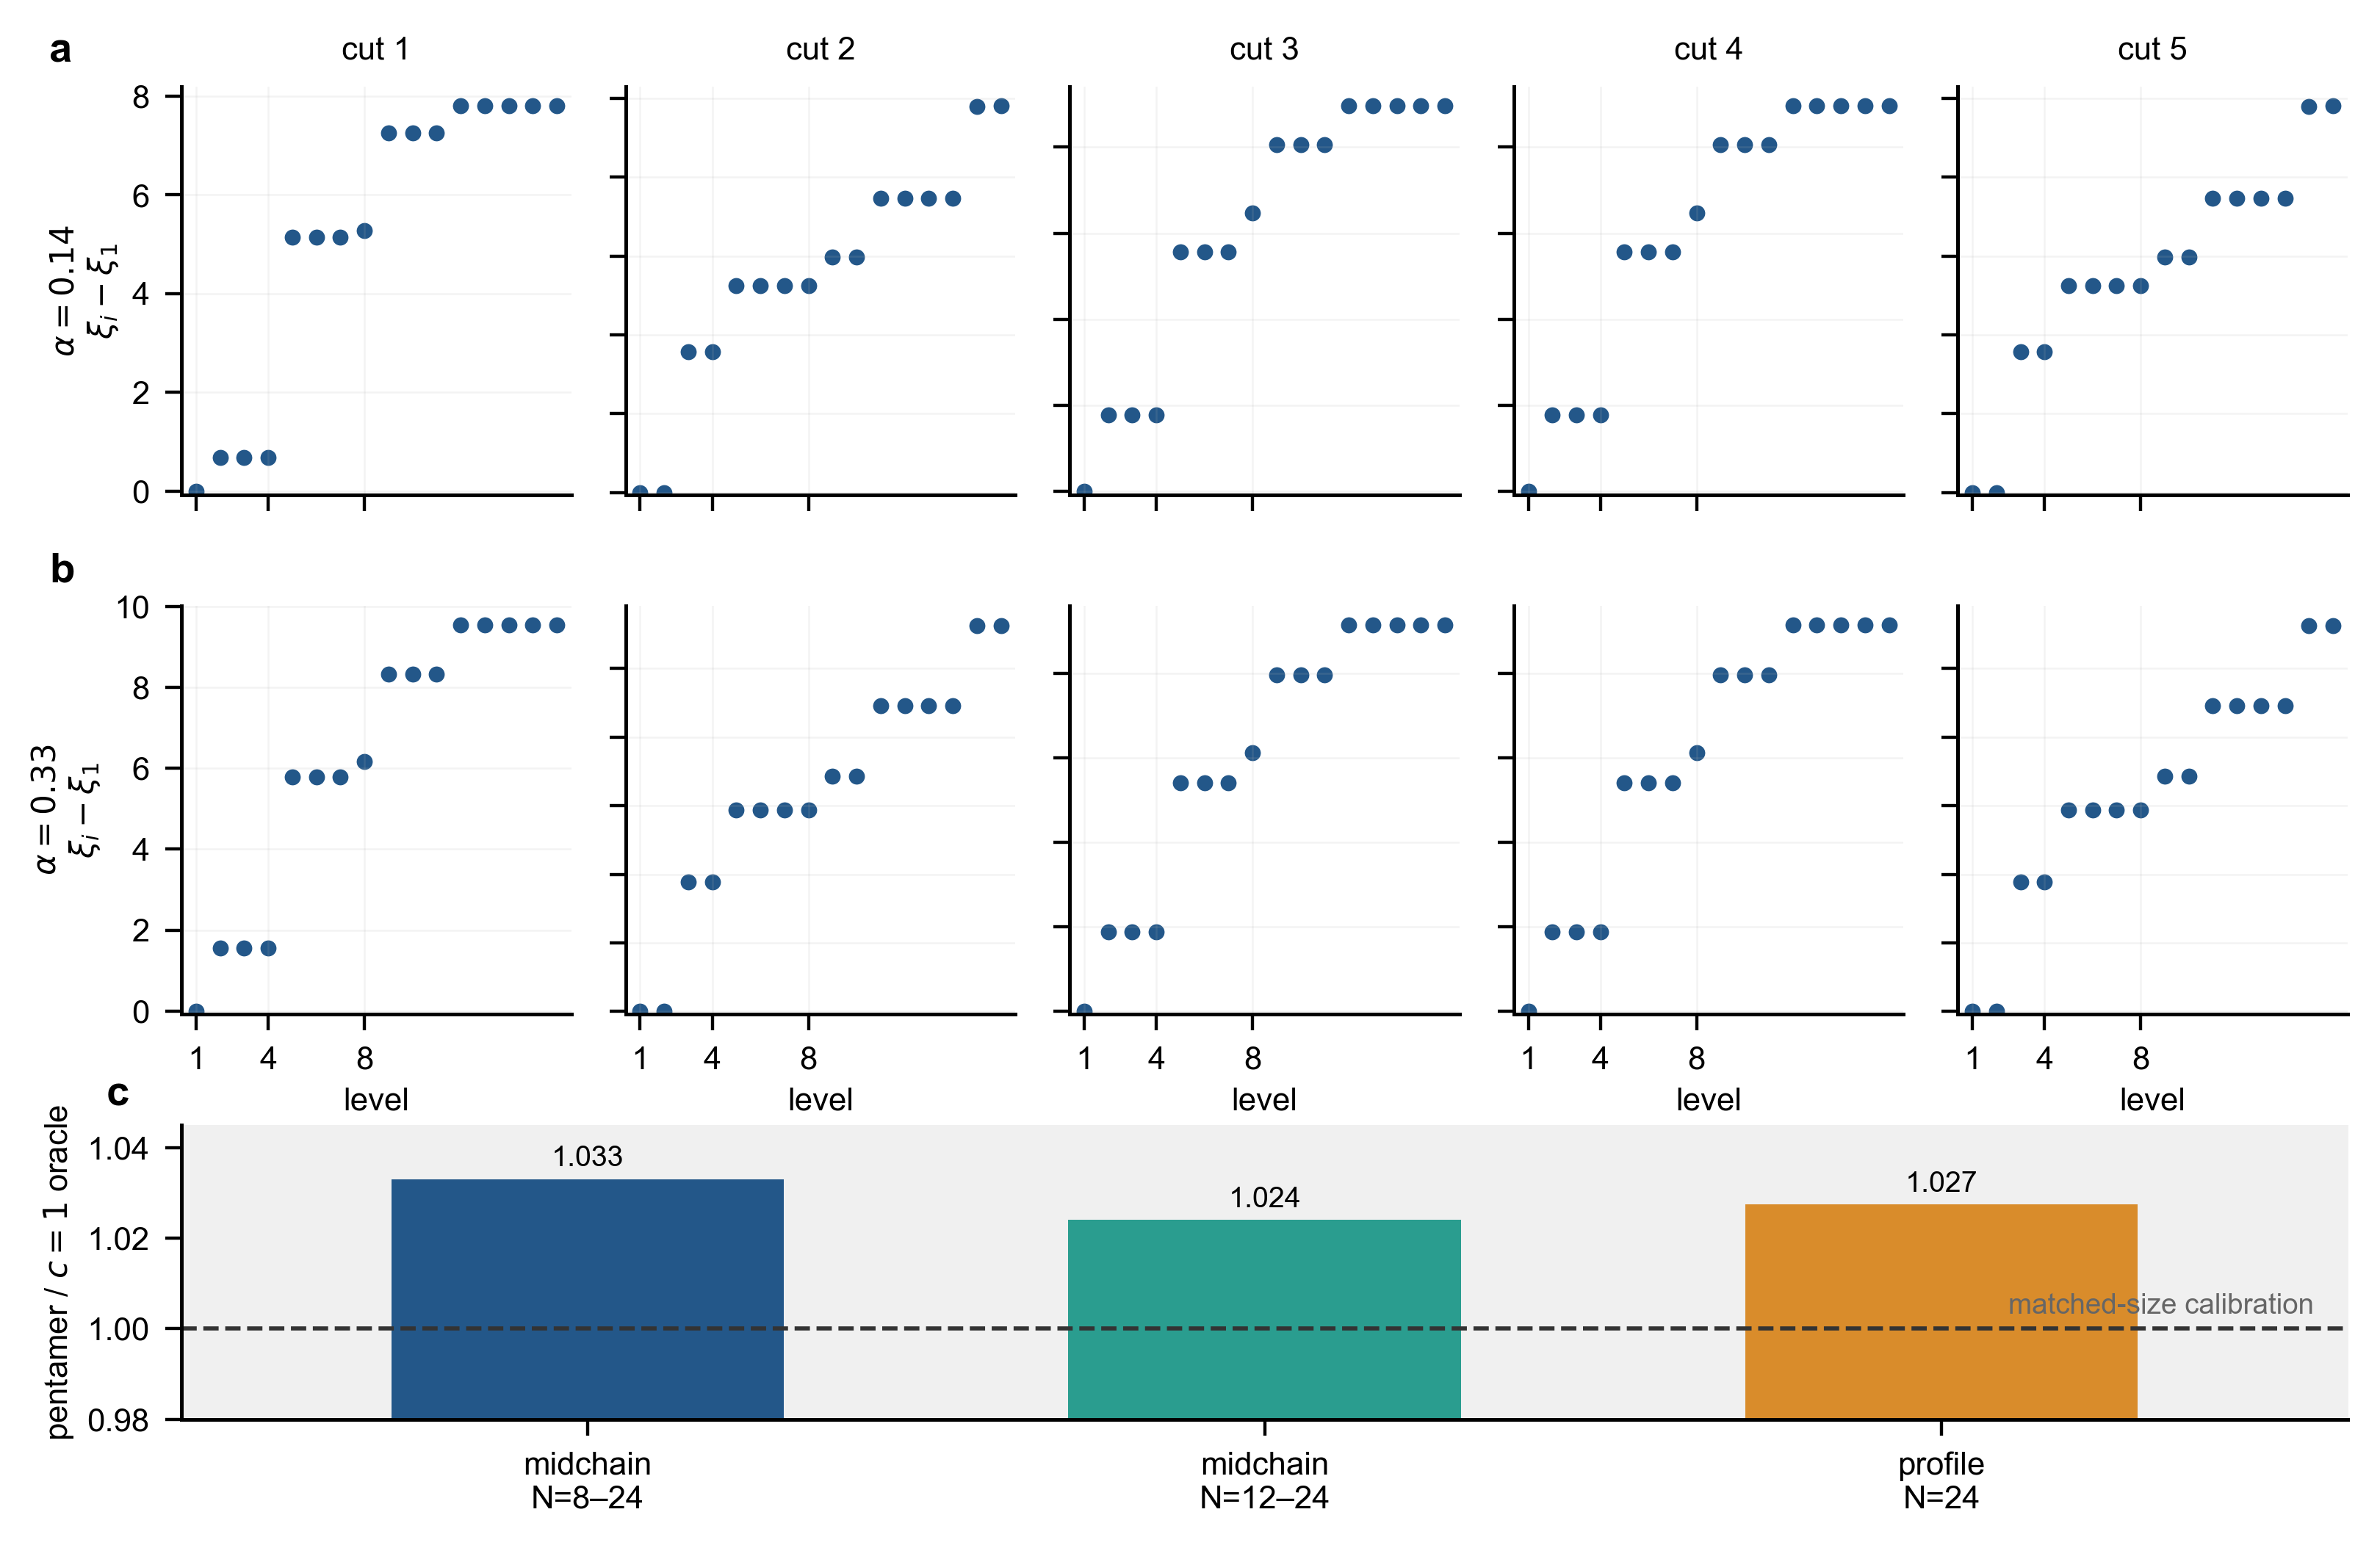
\includegraphics[width=0.94\textwidth]{fig4_entanglement.png}
  \caption{Entanglement and finite-size low-energy diagnostics.
  Five inequivalent bond classes are calibrated against a matched-size $c=1$ Heisenberg-chain oracle.
  The coefficient is interpreted only at the tested points.}
  \label{fig:entanglement}
\end{figure*}

\subsection{Reflection parity selects the visible local excitation}

The lowest excited doublet is not the lowest visible $q=\pi$ excitation.
Its projector-resolved spectral weight is below $4.6\times10^{-27}$ at the three representative positive-$\alpha$ points because the $q=\pi$ spin operator is even under reflection, whereas the target doublet is odd.
The lowest even-parity spin-$3/2$ multiplet carries weight 0.325--0.333, and all spin-$3/2$ multiplets together account for $84.1\%$--$97.6\%$ of the isolated-pentamer inelastic response.
This result identifies which local sector can contribute when collective states form, without assuming that the isolated multiplet remains a sharp quasiparticle at finite $\beta$.

\begin{figure*}[t]
  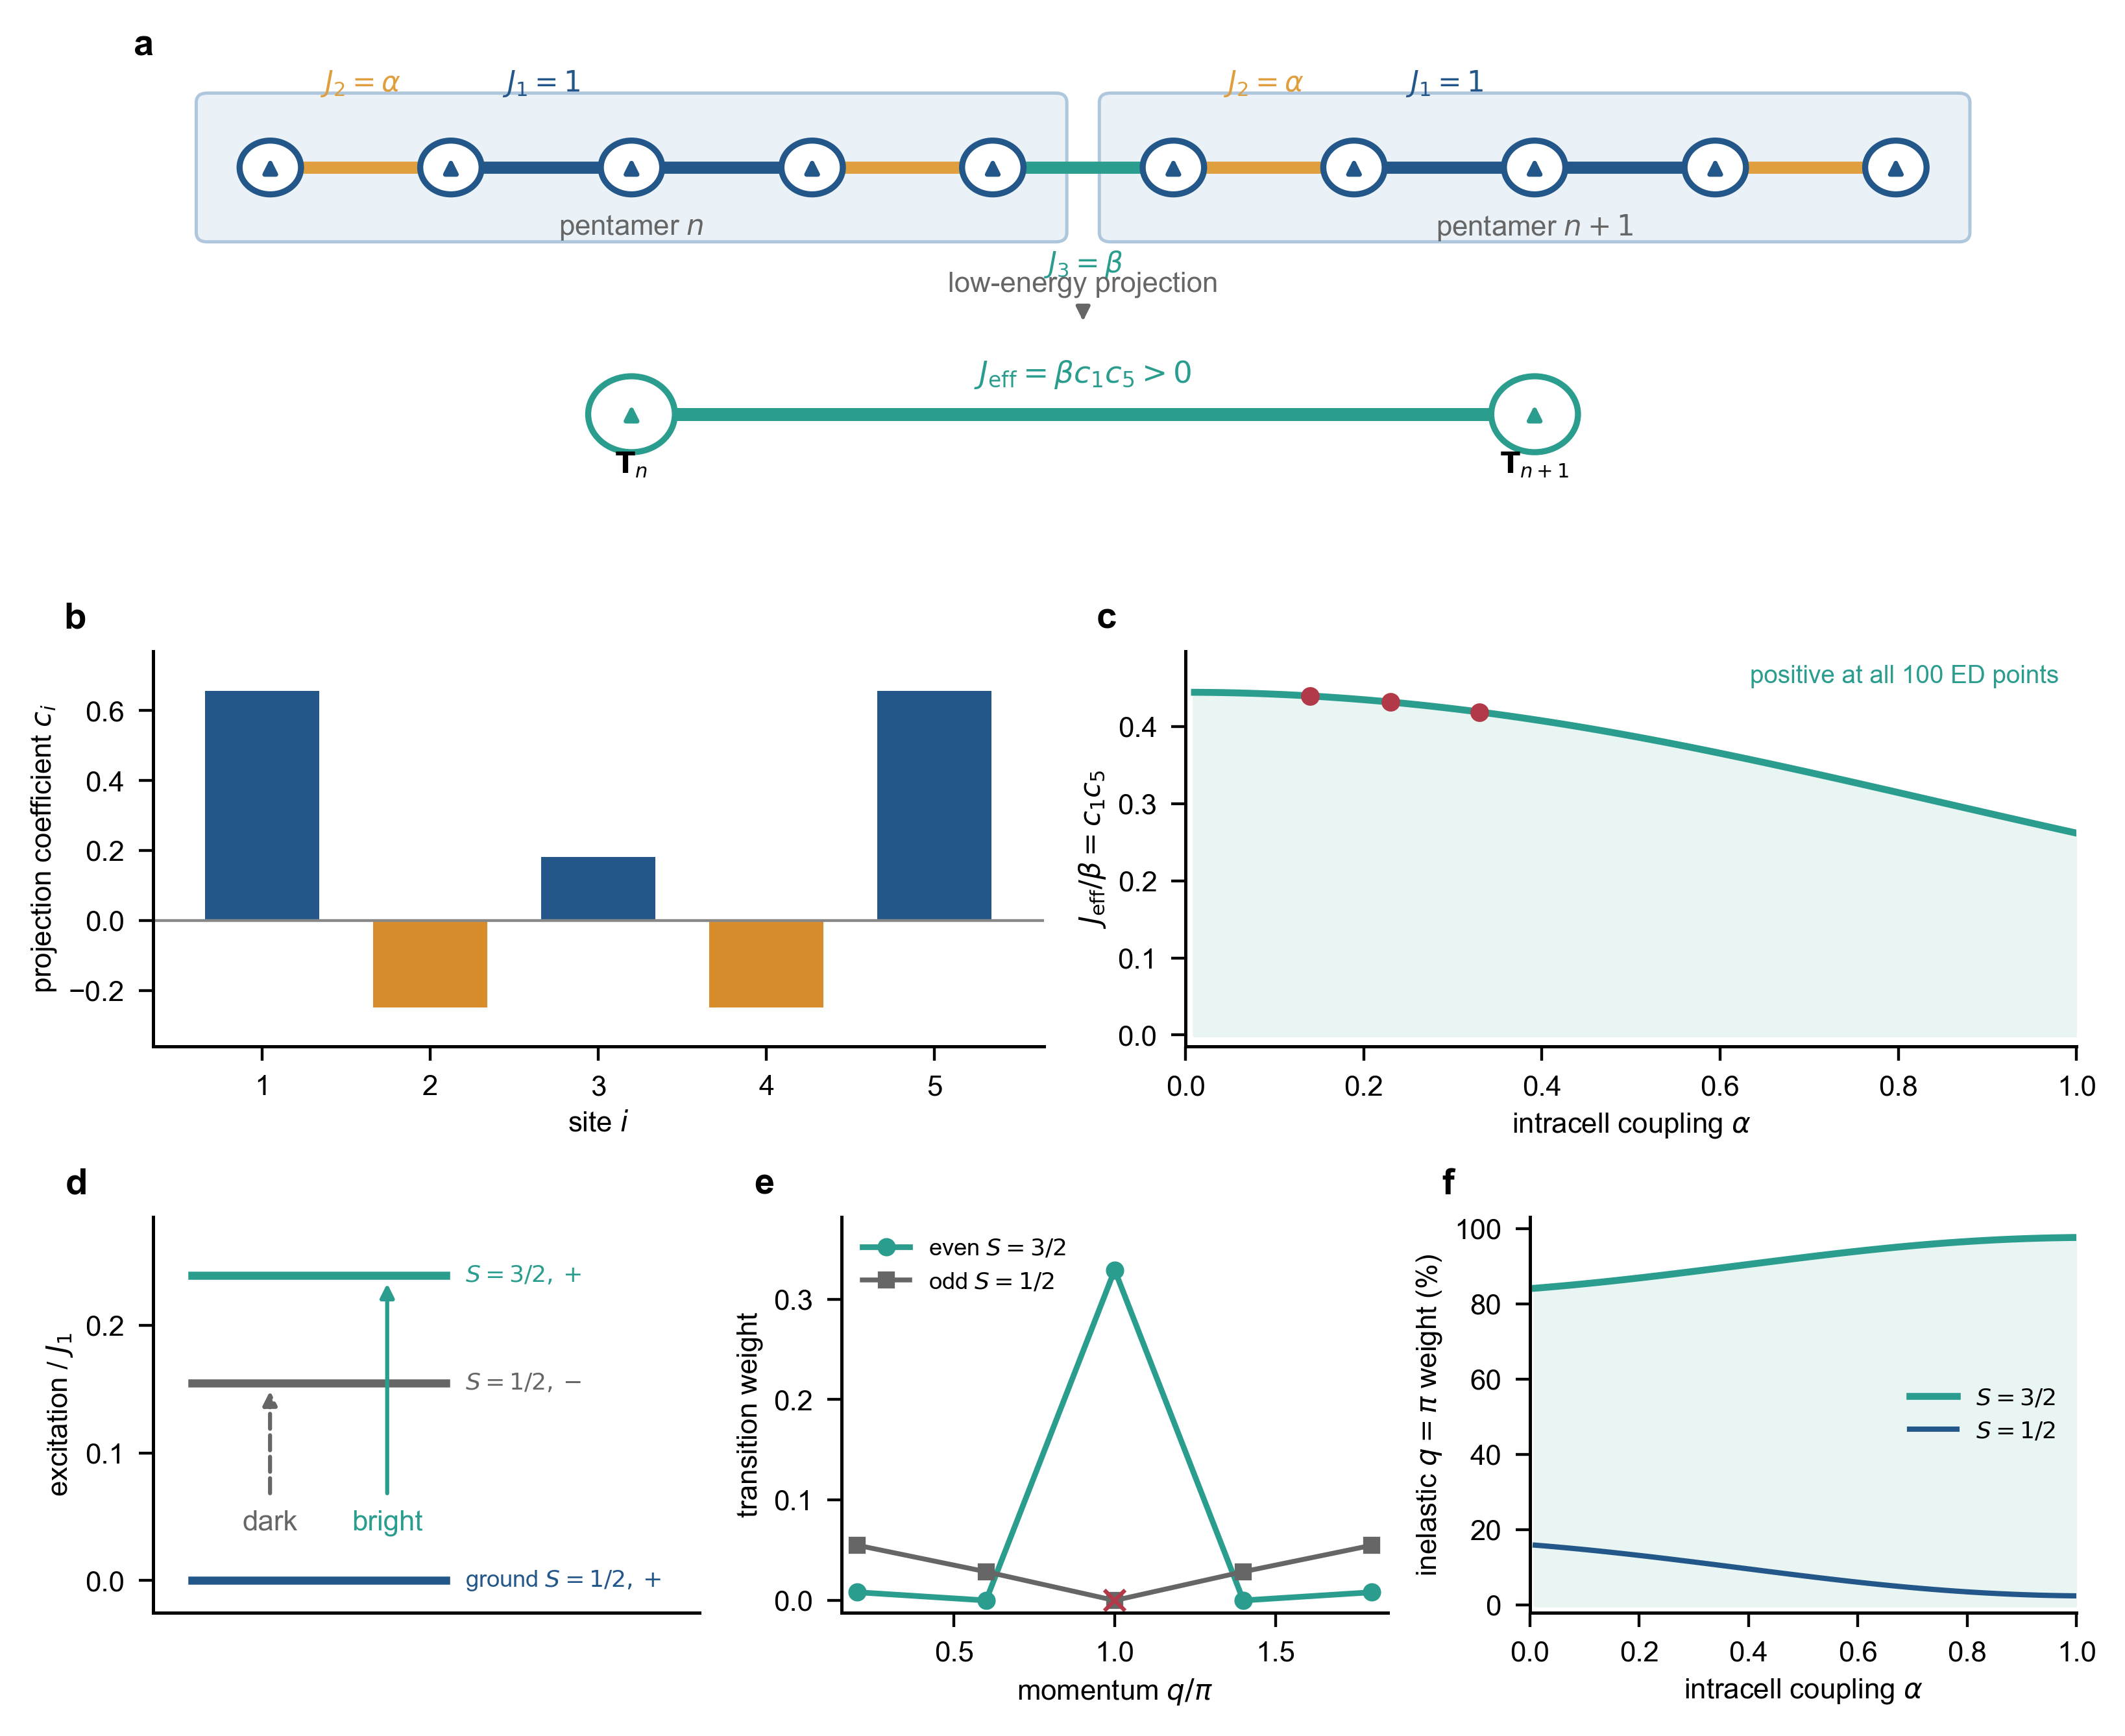
\includegraphics[width=0.92\textwidth]{fig5_selection_rules.png}
  \caption{Effective-chain continuum and local selection rules.
  The continuum bounds describe the weak-coupling effective chain, while the isolated-pentamer weights identify bright local spin-$3/2$ channels without assigning an unvalidated quasiparticle label.}
  \label{fig:selection}
\end{figure*}

\subsection{Collective dynamics confirms the pointwise spectral picture}

At $(\alpha,\beta,L,q)=(0.23,0.5,40,\pi)$, eleven accepted correction-vector frequencies cover $0\leq\omega/J_1\leq1.5$ and pass the peak-bracketing, spectral-weight, and residual gates.
The line shape agrees with the independently converged time-evolution result within the declared peak-position and integrated-weight budgets.

Full-momentum time evolution was completed at $(\alpha,\beta)=(1,1)$, $(1,0.1)$, and $(0.23,0.5)$.
All six individual runs and all three $\Delta t$/$\Delta t/2$ pairs passed.
The global and $q=\pi$ peak drifts are 0, 0, and $0.01J_1$ for the uniform, weak-coupling, and agreement points.
The corresponding low-frequency integrated-weight changes are $4.32\times10^{-5}$, $2.74\times10^{-5}$, and $1.97\times10^{-5}$.

The uniform point uses broadening $\eta=0.1$, whereas the weak-coupling and agreement points use $\eta=0.2$; all three use a spatial window of 18 sites.
We compare the spectral organization and time-step stability but do not compare weak-peak linewidths across different broadenings.

\begin{figure*}[t]
  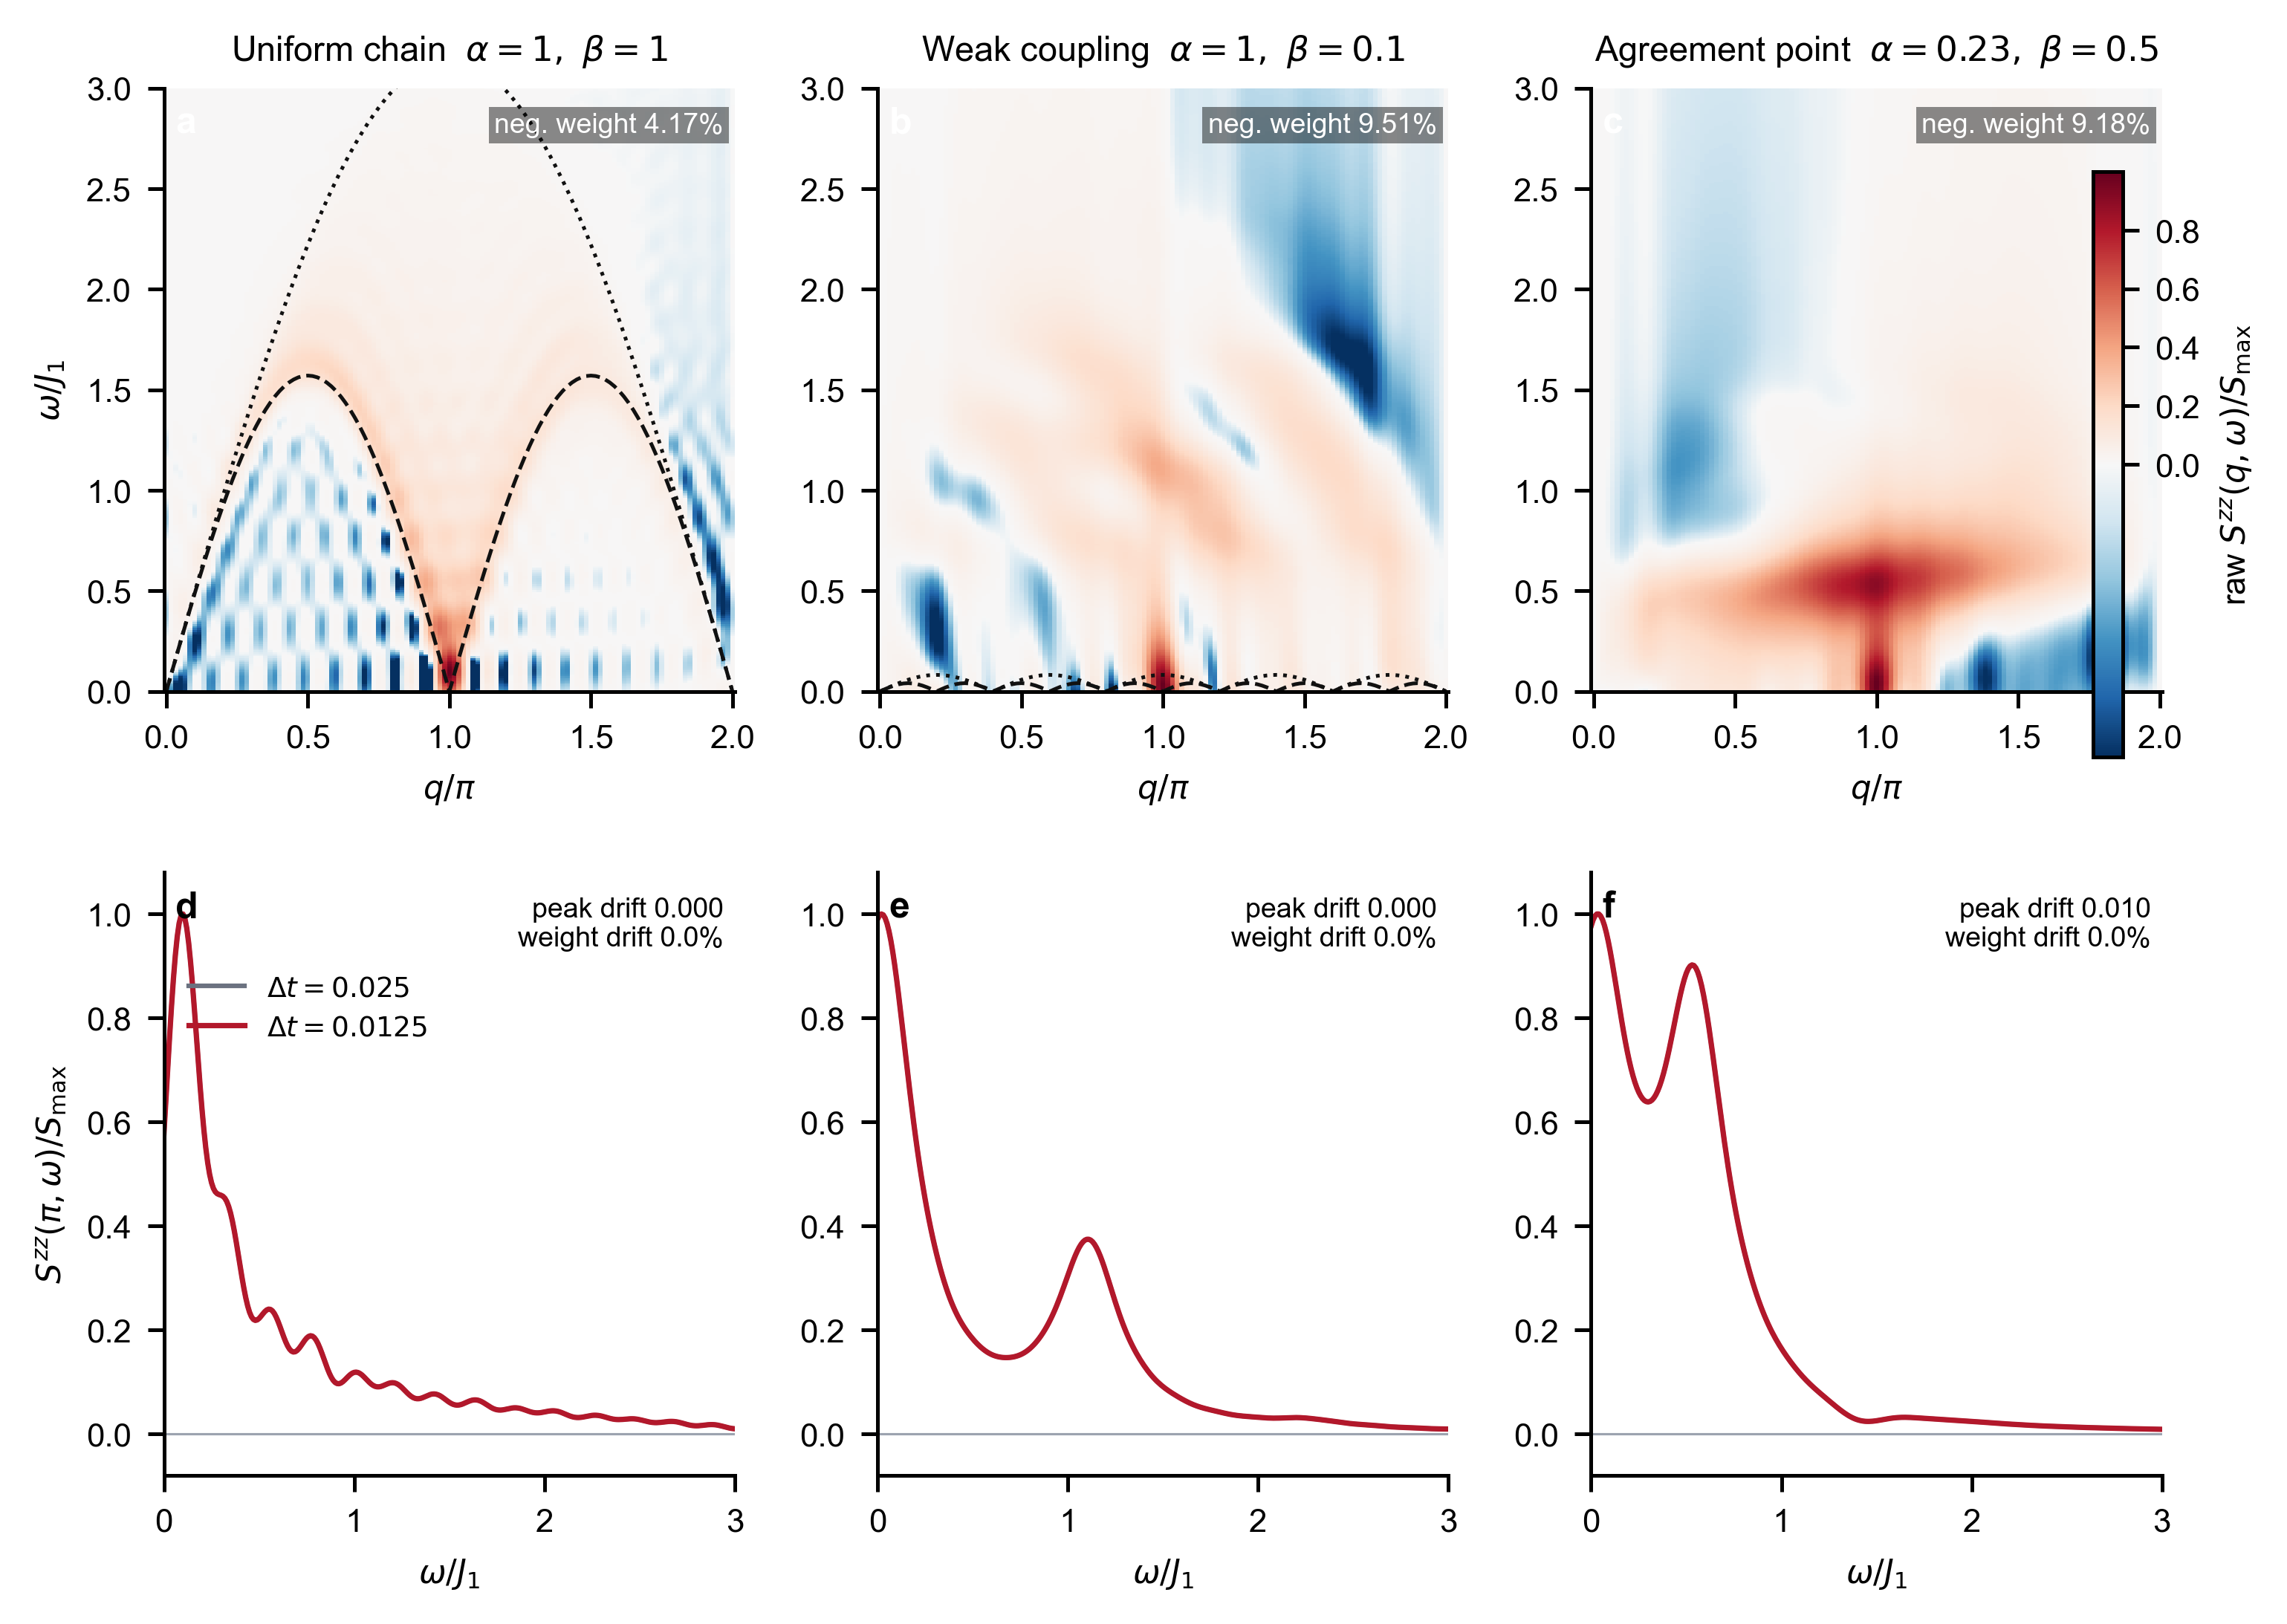
\includegraphics[width=0.97\textwidth]{fig6_fullq_dynamics.png}
  \caption{Raw full-momentum $\Szz$ and paired $q=\pi$ time-step slices at three representative positive-coupling points.
  Negative Fourier ringing is shown rather than clipped.
  All six runs and all three $\Delta t$/$\Delta t/2$ pairs pass the spectral gates.}
  \label{fig:fullq}
\end{figure*}

\begin{figure}[t]
  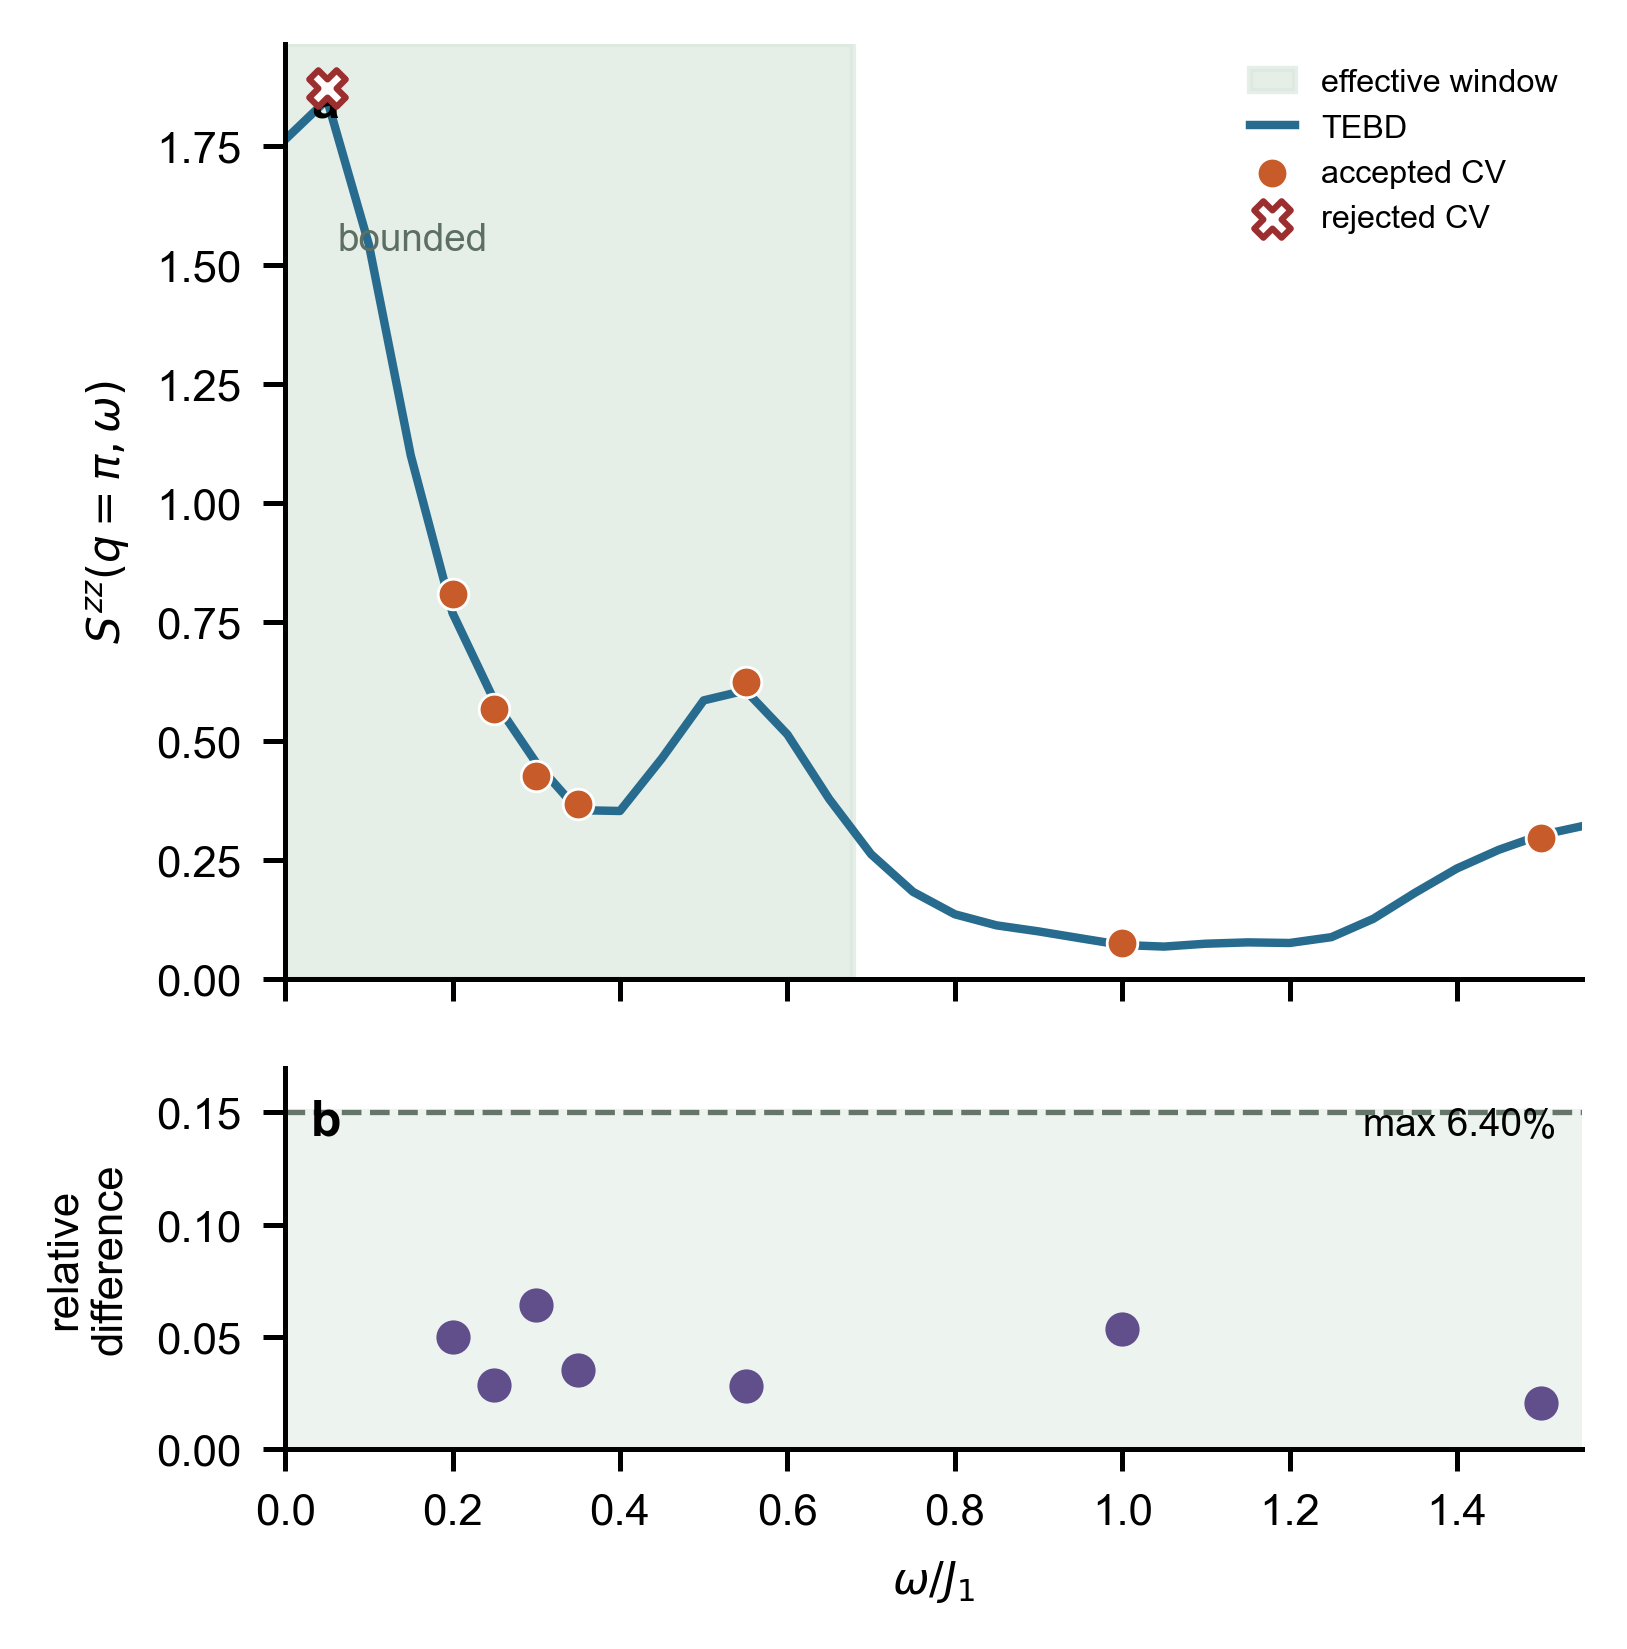
\includegraphics[width=\columnwidth]{fig7_cv_tebd.png}
  \caption{Pointwise correction-vector and time-evolution comparison at $\alpha=0.23$, $\beta=0.5$, $L=40$, and $q=\pi$.
  Eleven accepted frequencies bracket the principal feature and cover $0\leq\omega/J_1\leq1.5$.}
  \label{fig:cv-tebd}
\end{figure}

\subsection{Negative intra-cell exchange reconstructs the finite-size momentum}

The negative-$\alpha$ data show a reproducible change in the dominant structure-factor momentum.
Deep in the scanned region, $\qpeak\simeq0.60\pi$; closer to $\alpha=0$, the maximum locks to $q=\pi$.
The local multiplet structure offers a candidate explanation for the deep-region value.
At all 201 sampled points with $-1\leq\alpha\leq-0.001$, the isolated pentamer has a spin-$3/2$ ground multiplet rather than the spin-$1/2$ doublet found for $\alpha>0$.
Projecting the intra-cell couplings onto that quartet and evaluating the single-spin shape factor at three representative momenta gives a positive effective exchange $\Jeff/\beta=0.1075$--$0.1111$, with the $q=0.60\pi$ weight in the range 0.62--0.73 while the $q=\pi$ weight never exceeds $1.3\times10^{-2}$ on the same scale.
The projector identities are satisfied to $3.1\times10^{-16}$ and the dominant folded momentum is $0.60\pi$ without exception.
This is a local single-cell statement: it shows that the deep-region momentum scale is already selected by the isolated quartet, but it does not establish that the chain orders there.

Stage B evaluated 96 parameter--size records at 48 coupling points.
Eighty-nine records passed the Practical V2 gates, while seven non-boundary records remained bounded and were excluded from accepted-only inference.

The accepted-only analysis identified eight candidate intervals across seven $\beta$ slices.
Stage C evaluated these intervals with 29 additional $L=60,80$ cells at 64 sweeps.
All 29 cells passed the remote parent and child checksums, non-overwriting transfer, local checksum, and independent validator.
Seven of eight targets retain either a momentum reconstruction or a sign change in $\Delta R=R_{80}-R_{60}$ that satisfies its declared diagnostic criterion.
No adjacent interval carries both signatures.
Only the $\beta=0.05$ momentum interval reaches the target width 0.025, and the $\beta=0.10$ slice supplies no supported internal interval at the final size pair.

The data establish a finite-size momentum reconstruction but do not locate a joint thermodynamic boundary.
The mismatch is compatible with a broad crossover, a slowly converging incommensurate regime, or residual finite-size effects.

\begin{figure}[t]
  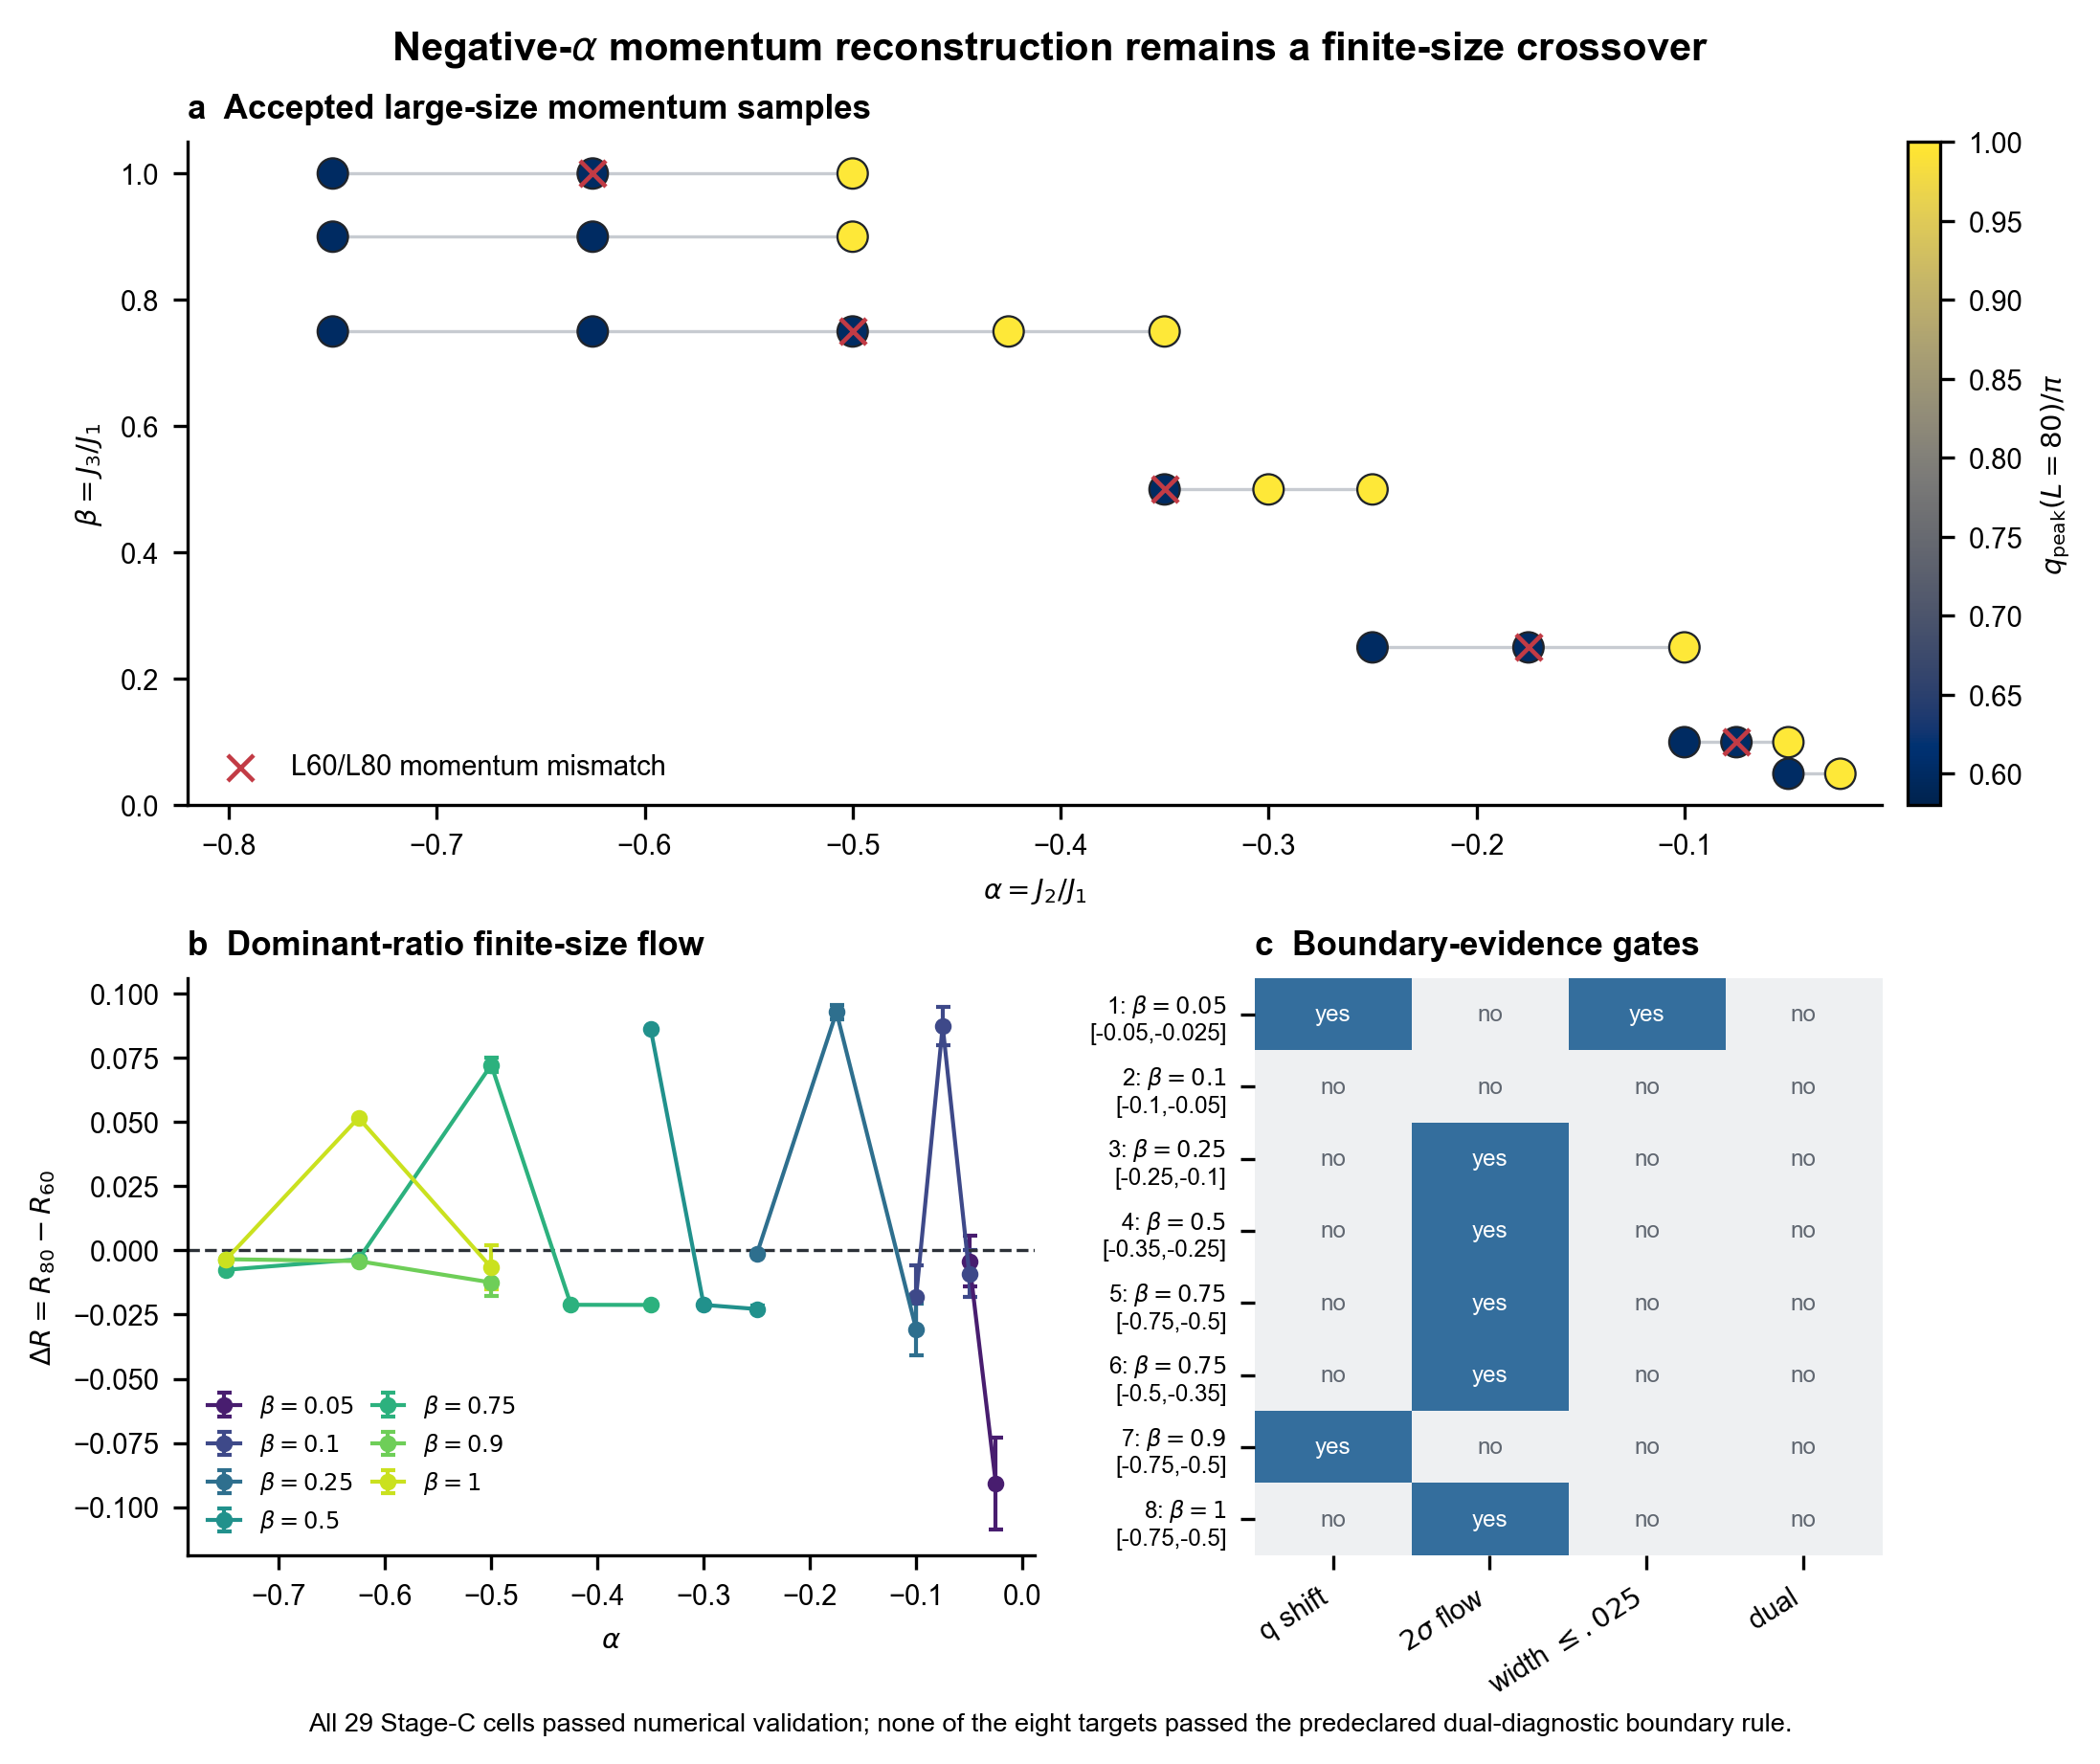
\includegraphics[width=\columnwidth]{fig8_negative_reconstruction.png}
  \caption{Accepted-only negative-$\alpha$ momentum reconstruction.
  Large-size data move from $\qpeak\simeq0.60\pi$ to $\pi$, but the momentum and dominant-ratio diagnostics do not select the same adjacent interval.}
  \label{fig:negative-reconstruction}
\end{figure}

\subsection{Saved-state diagnostics and terminal solver control}

Six additional points were evaluated with saved $L=80$ ground-state wavefunctions using two $S^z=0$ initial states and 64 sweeps per initial state.
The points were $\alpha=-0.25,-0.175,-0.10$ at $\beta=0.25$ and $\alpha=-0.625,-0.50,-0.425$ at $\beta=0.75$.
All parent runs passed the Practical V2 gates, with a largest variance per site of $1.2875\times10^{-9}$.

At $\beta=0.25$, the earlier $L=80$ audit gave $\ceff=0.467$--0.605 at $\alpha=-0.10$, compared with 0.886--0.971 at $\alpha=-0.175$ and 0.981--1.049 at $\alpha=-0.25$.
The three $\beta=0.75$ points gave 0.905--0.976.
These ranges measure sensitivity to the fitting window and initialization; they are not confidence intervals.

A subsequent size comparison used $L=40,60,80$ at $\alpha=-0.175,-0.150,-0.125,-0.100$ and $\beta=0.25$.
At $\alpha=-0.10$, the ten-intercept coefficients span 0.970--1.340, 0.625--0.959, and 0.467--0.605 with increasing length.
At fixed window $f=0.20$, the dual-start mean decreases from 0.988 to 0.695 and 0.533.
That decrease, however, is not a converged finite-size trend.
The whole sequence was computed with the historical Krylov setting, and only its $L=80$ endpoint has a $k=8$ control.
At that point the period-10, $f=0.20$ coefficient moves from 0.582 to 0.932 (\texttt{center}) and from 0.484 to 0.932 (\texttt{ferro\_j2}), after which the two initial states agree to $3.4\times10^{-8}$.
A solver setting that shifts an endpoint by this amount cannot support a size-scaling reading of the sequence, and the $L=40$ and $L=60$ records have no equivalent control.

\begin{figure}[t]
  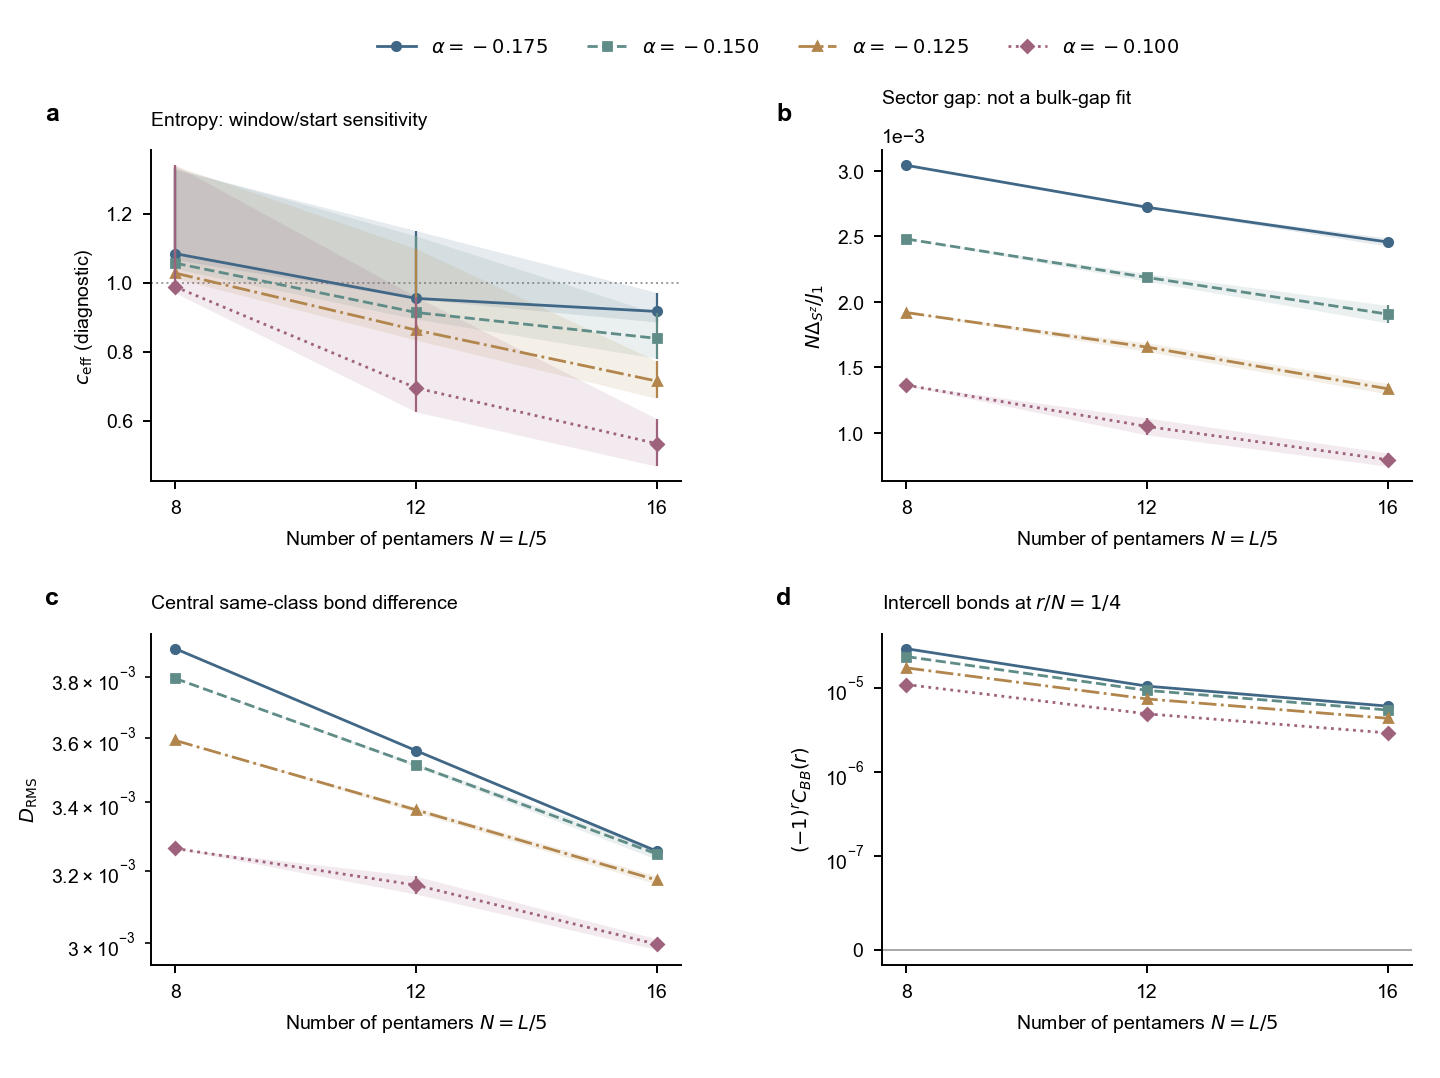
\includegraphics[width=\columnwidth]{fig9_negative_size_evidence.png}
  \caption{Joint finite-size evidence near the negative-$\alpha$ anomaly.
  Entropy coefficients, bond-class variation, connected correlations, and sector gaps are shown together to expose size and initialization sensitivity.
  All panels use the historical solver setting; the $k=8$ control applies only to the $L=80$, $\alpha=-0.10$ endpoint and is not propagated through this figure.}
  \label{fig:negative-size}
\end{figure}

The terminal Krylov control identifies which part of this anomaly was numerical.
The earlier $k=3\rightarrow8$ change strongly revised some entropy slopes at $\alpha=-0.10$, showing that the old solver setting was not stable.
By contrast, the final $k=8\rightarrow12$ comparison at the same $L=80$ point is stable to the small absolute differences reported in Sec.~\ref{sec:methods} and leaves $\qpeak=\pi$.
This makes the accepted $L=80$ observables at that point robust against a further increase of the Krylov subspace.
It does not supply a $\chi$ series, larger sizes, or a thermodynamic order parameter.
